\documentclass[12pt,a4paper]{article}

\usepackage[margin=1in]{geometry}
\usepackage{graphicx}
\usepackage{hyperref}
\usepackage{listings}
\usepackage{booktabs}
\usepackage{float}
\usepackage{subcaption}
\usepackage{parskip}

% --- CODE STYLE ---
\lstset{
    basicstyle=\ttfamily\small,
    breaklines=true,
    frame=single,
    numbers=left,
    numberstyle=\tiny,
    tabsize=4,
    showstringspaces=false
}

\hypersetup{colorlinks=true, urlcolor=blue, linkcolor=black}

% ===========================
\begin{document}

% --- TITLE PAGE ---
\begin{titlepage}
    \centering
    \vspace*{2cm}
    {\Huge\textbf{GameCraft}}\\[0.4cm]
    {\large A Minecraft-Themed Multi-Game Hub}\\[2cm]
    {\Large CS108 --- Systems \& Software Lab}\\[0.3cm]
    {\large Project Report}\\[2cm]
    \begin{tabular}{ll}
        \textbf{Authors:} & Akshita Jain \quad (25B0999) \\[0.3cm]
                          & Maulik Jain \quad (25B1002) \\[1cm]
        \textbf{Date:}    & \today
    \end{tabular}
    \vfill
    Department of Computer Science and Engineering\\
    IIT Bombay
\end{titlepage}

\tableofcontents
\newpage

% ==========================
\section{External Libraries Used}
% ==========================

\begin{center}
\renewcommand{\arraystretch}{1.4}
\begin{tabular}{lp{10cm}}
\toprule
\textbf{Library} & \textbf{Purpose} \\
\midrule
\texttt{pygame}     & Core graphics and audio library. Handles window creation, event polling, sprite and font rendering, image loading, and audio playback via \texttt{pygame.mixer}. \\
\texttt{numpy}      & Represents game boards as 2D arrays and evaluates win conditions via vectorised array slicing without manual loops. \\
\texttt{matplotlib} & Generates post-match charts: a pie chart of game popularity and a bar chart of top players by wins, saved as PNGs and loaded back into Pygame. \\
\texttt{sys}        & Provides \texttt{sys.argv} to receive authenticated player names from the Bash entry point, and \texttt{sys.exit()} for clean termination. \\
\texttt{os}         & Constructs cross-platform paths, invokes Bash subprocesses via \texttt{os.system()}, and checks file existence with \texttt{os.path.exists()}. \\
\texttt{math}       & Supplies \texttt{math.sqrt()} and trigonometric functions used in rendering. \\
\texttt{csv}        & Parses \texttt{history.csv} for cumulative win/loss records appended after every game session. \\
\bottomrule
\end{tabular}
\end{center}

% ==========================
\section{Features Implemented}
% ==========================

\subsection{Authentication System (Bash)}

The application launches exclusively through \texttt{main.sh}, enforcing two-player authentication before any game session begins.

\begin{itemize}
    \item \textbf{SHA-256 Password Hashing:} Passwords are never stored in plaintext; they are hashed with \texttt{sha256sum} and compared against \texttt{users.tsv}.
    \item \textbf{Registration:} If a username is not found, the user is prompted to register; a new tab-separated entry is appended to \texttt{users.tsv}.
    \item \textbf{Uniqueness Constraint:} Both players must authenticate as different users; Player 2 is re-prompted on a duplicate login.
    \item \textbf{Argument Passing:} On successful dual-login, \texttt{python3 game.py \$PLAYER1 \$PLAYER2} is invoked, passing authenticated usernames as command-line arguments.
\end{itemize}

\subsection{Main Hub (Python / Pygame)}

The Pygame engine presents a Minecraft-themed graphical hub with multiple screens.

\begin{itemize}
    \item \textbf{Start Screen:} Displays the ``GameCraft'' title and both player names. Each player selects a Minecraft character avatar (Zombie, Pig, Dog, or Steve) from side panels before proceeding.
    \item \textbf{Game Menu:} Lists three playable games and a League mode; navigation back to the start screen is available.
    \item \textbf{How to Play:} A dedicated screen with instructions overlaid on a thematic background image.
    \item \textbf{Statistics Screen:} Displays Matplotlib-generated charts (game popularity pie chart, top-players bar chart) loaded as Pygame surfaces.
    \item \textbf{Leaderboard Screen:} Players select a game and sort method (Total Wins, Total Losses, W/L Ratio) and trigger a formatted terminal display via \texttt{leaderboard.sh}.
\end{itemize}

\begin{figure}[H]
    \centering
    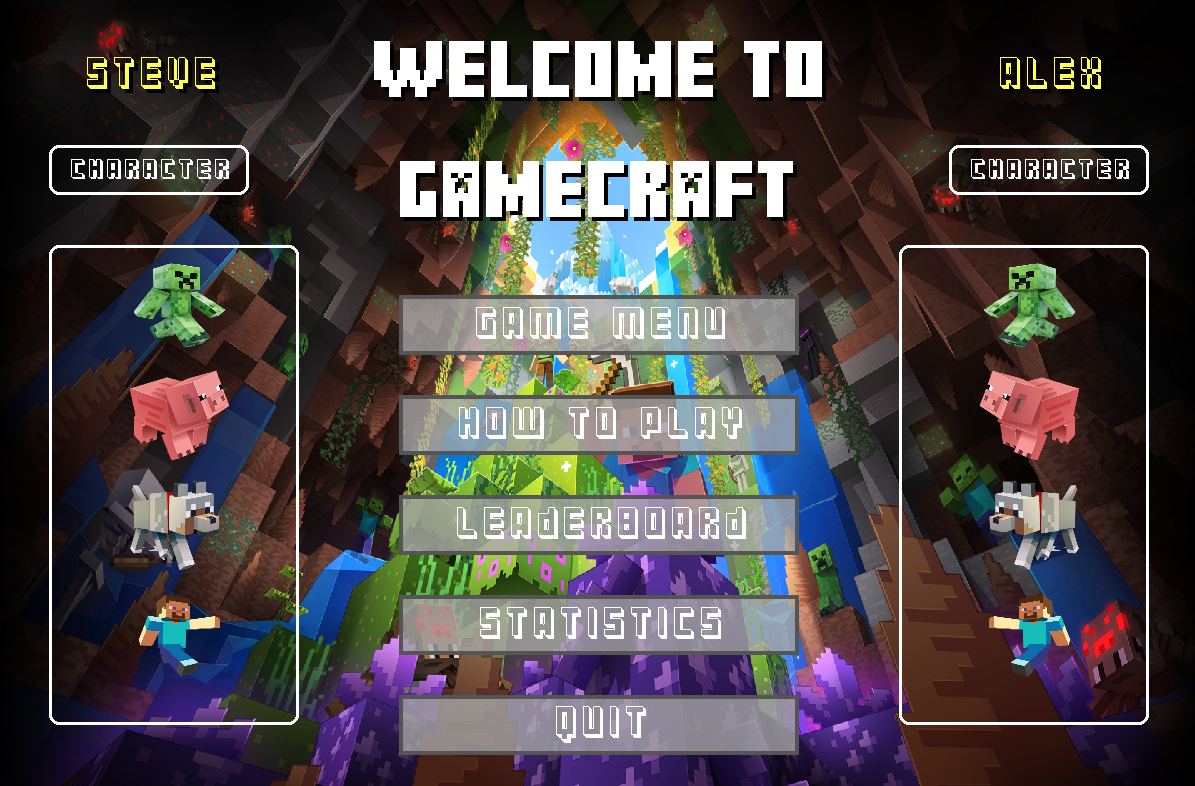
\includegraphics[width=0.72\textwidth]{figures/start_screen.png}
    \caption{Start Screen --- ``Welcome to GameCraft'' with avatar selection panels}
\end{figure}

\subsection{Game: Tic-Tac-Toe}

Played on a $10\times10$ board; 5 consecutive marks are required to win.

\begin{itemize}
    \item Players place Diamond (Player 1) and Golden Apple (Player 2) sprites alternately.
    \item Win conditions checked horizontally, vertically, and diagonally using NumPy slicing.
    \item A win triggers an animated line drawn through the winning sequence.
    \item Ghost piece previews shown on hover before placement.
\end{itemize}

\subsection{Game: Othello (Reversi)}

Standard $8\times8$ board with classic Othello rules.

\begin{itemize}
    \item The board initialises with two Black and two White discs at the centre.
    \item Valid move detection searches all 8 directions for opponent pieces that would be flanked.
    \item All flanked opponent pieces are flipped on a valid move.
    \item A player's turn is skipped if they have no valid moves; the game ends when neither player can move.
\end{itemize}

\subsection{Game: Connect Four}

$7\times7$ vertical grid with gravity-based piece dropping.

\begin{itemize}
    \item Players drop Diamond vs.\ Emerald sprites; pieces fall to the lowest available row.
    \item Win detection checks for 4 in a row horizontally, vertically, and diagonally via NumPy.
    \item Ghost piece preview and a mid-game pause screen are available.
\end{itemize}

\begin{figure}[H]
    \centering
    \begin{subfigure}[b]{0.48\textwidth}
        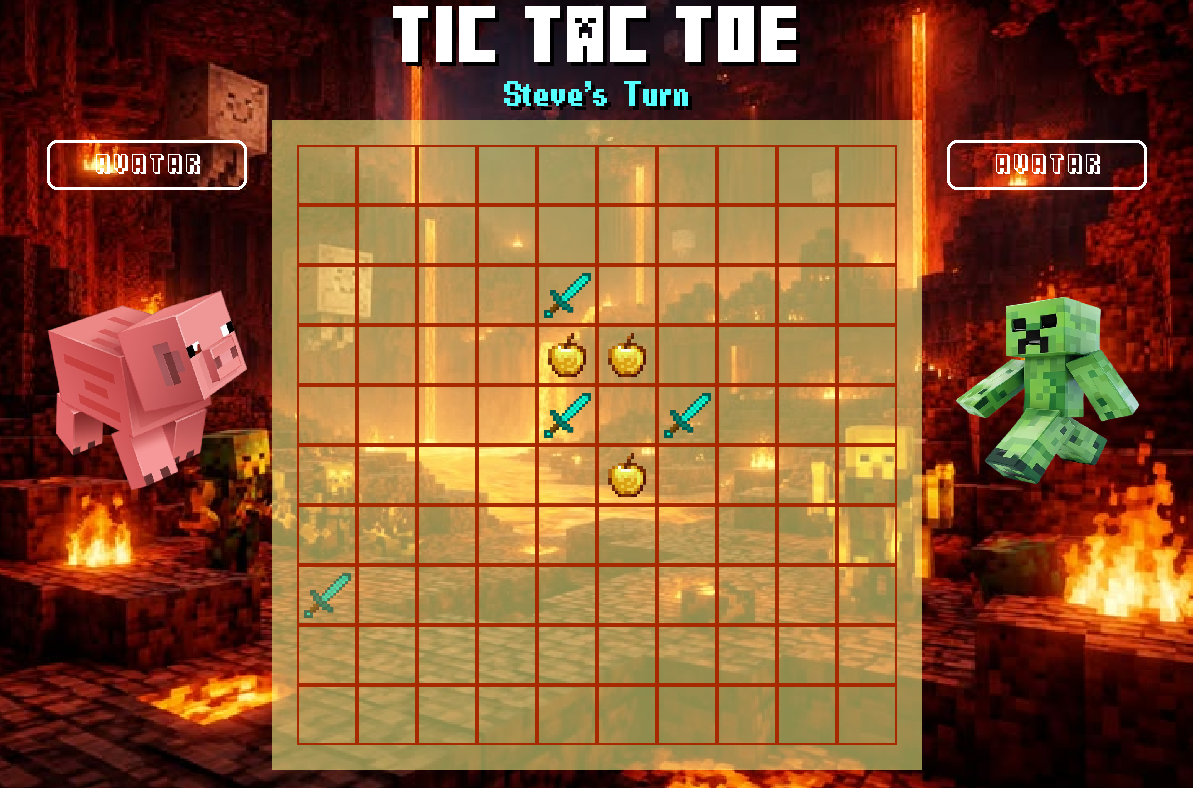
\includegraphics[width=\textwidth]{figures/tictactoe.png}
        \caption{Tic-Tac-Toe (10$\times$10 board)}
    \end{subfigure}
    \hfill
    \begin{subfigure}[b]{0.48\textwidth}
        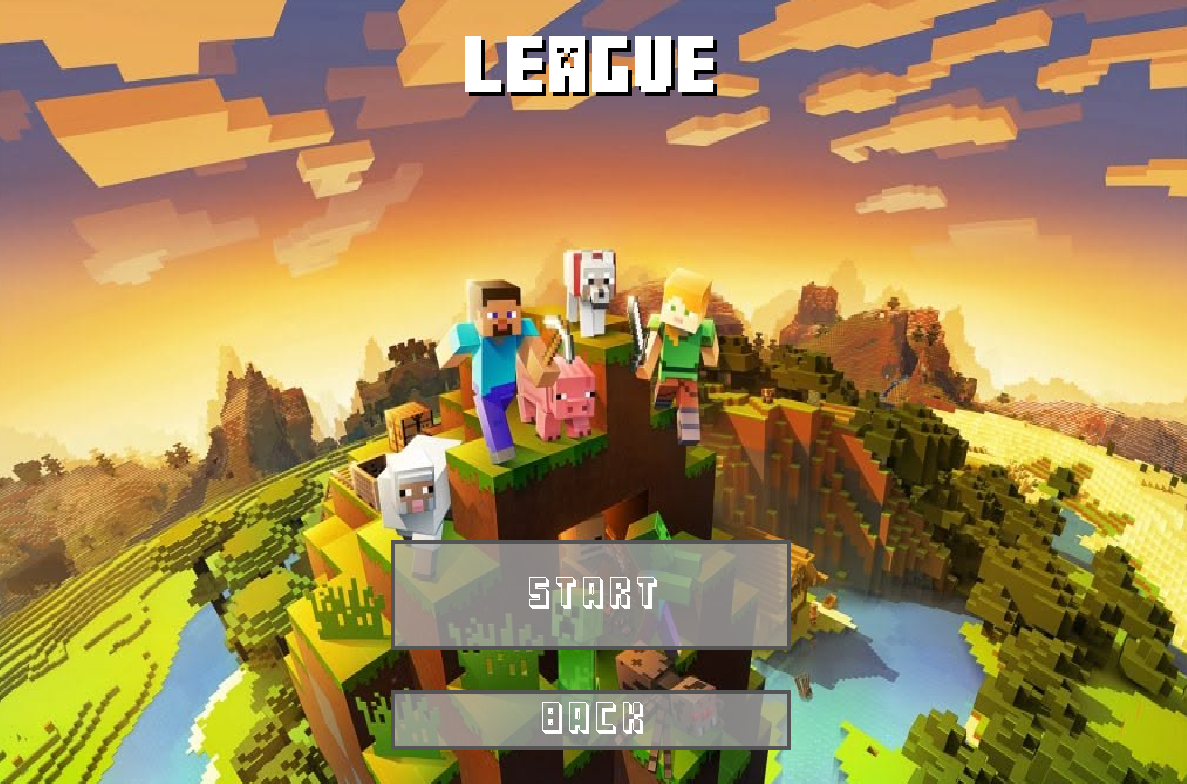
\includegraphics[width=\textwidth]{figures/league.png}
        \caption{League mode start screen}
    \end{subfigure}
    \caption{In-game screens}
\end{figure}

\subsection{League Mode}

Runs all three games sequentially in a single session.

\begin{itemize}
    \item Results of Tic-Tac-Toe, Othello, and Connect 4 are tallied.
    \item The player with more individual game wins is declared the League Champion.
    \item A final champion screen displays the score (e.g.\ 2--1) and the winner's name.
\end{itemize}

\subsection{Leaderboard \& Analytics}

\begin{itemize}
    \item \texttt{update\_history()} in \texttt{game.py} appends results to \texttt{history.csv} after each match.
    \item \texttt{leaderboard.sh} operates in two modes: \texttt{update} (writes new records) and \texttt{display} (sorts and renders a terminal table via \texttt{column -t}).
    \item Matplotlib refreshes a game-popularity pie chart and a top-players bar chart after every match.
\end{itemize}

\begin{figure}[H]
    \centering
    \begin{subfigure}[b]{0.48\textwidth}
        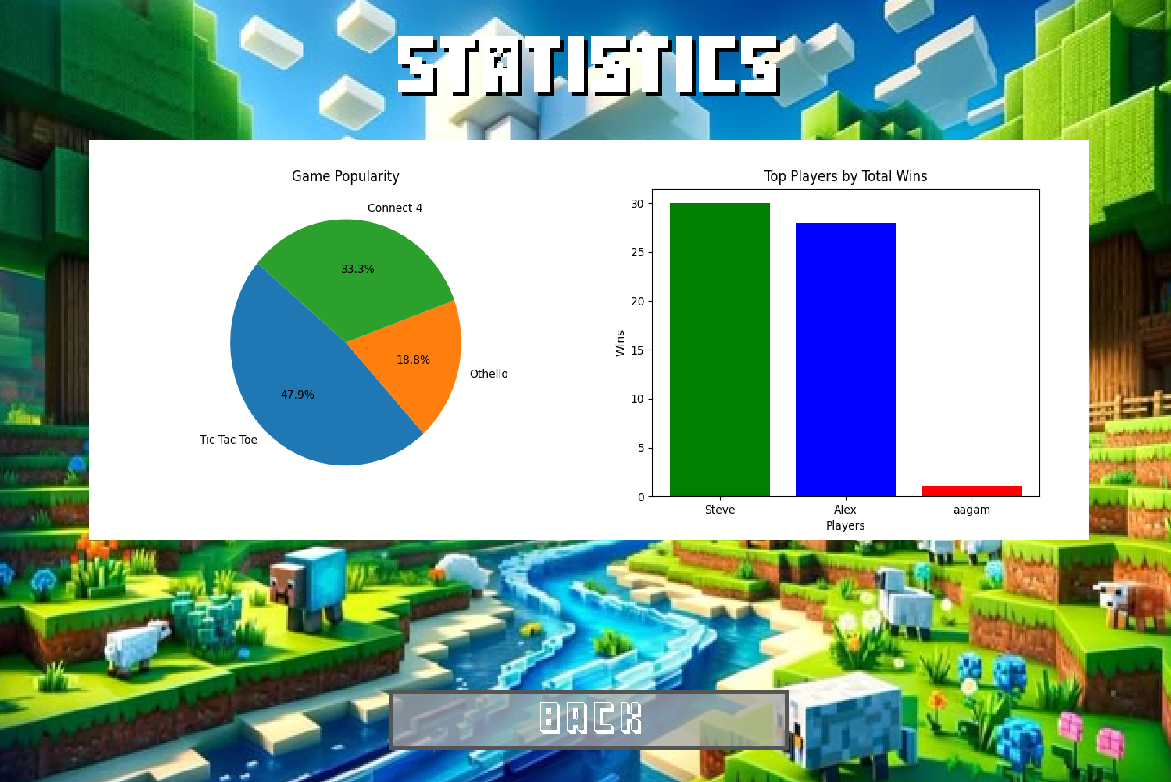
\includegraphics[width=\textwidth]{figures/statistics.png}
        \caption{Statistics screen (Matplotlib charts)}
    \end{subfigure}
    \hfill
    \begin{subfigure}[b]{0.48\textwidth}
        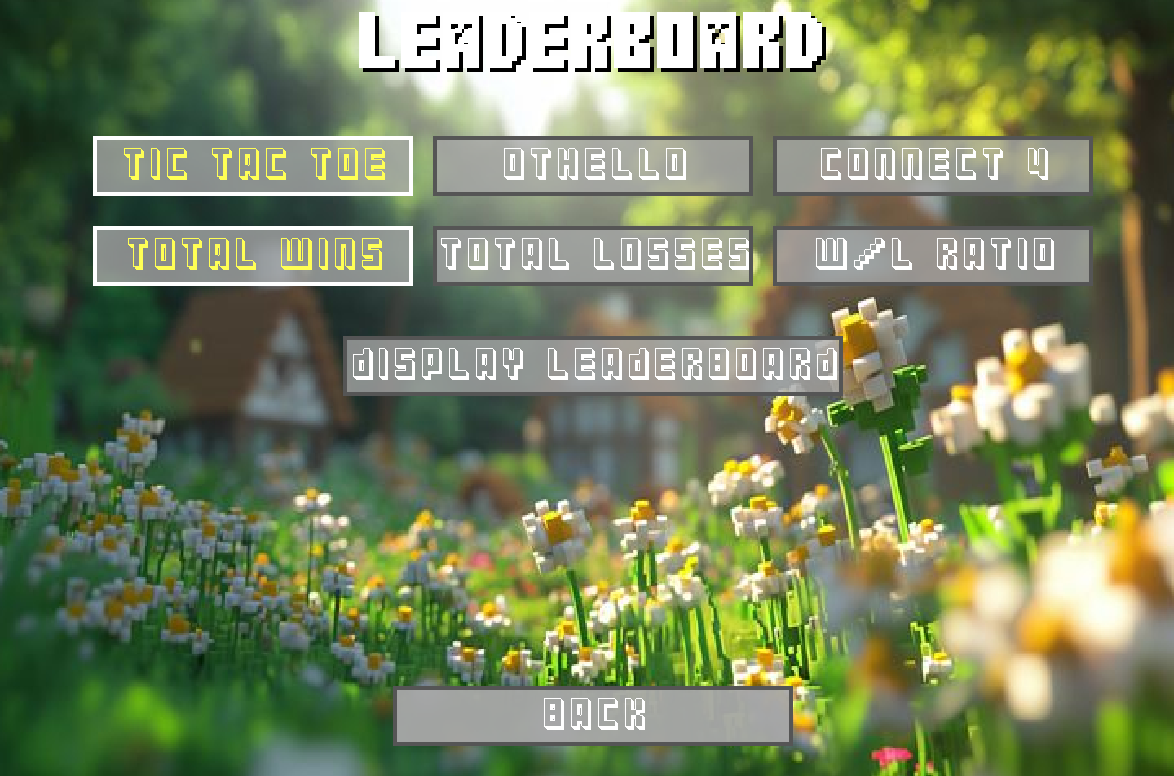
\includegraphics[width=\textwidth]{figures/leaderboard.png}
        \caption{Leaderboard selection screen}
    \end{subfigure}
    \caption{Analytics and leaderboard screens}
\end{figure}

\newpage

% ==========================
\section{Code Logic}
% ==========================

\subsection{Generic \texttt{Game} Base Class (\texttt{game.py})}

The \texttt{Game} class is the abstract foundation inherited by all three game modules.

\begin{lstlisting}[language=Python, caption={Game base class structure}]
class Game:
    def players(self):
        self.p1 = sys.argv[1] if len(sys.argv) > 1 else "Steve"
        self.p2 = sys.argv[2] if len(sys.argv) > 2 else "Alex"

    def switch_turns(self):
        self.player *= -1   # Player 1 = 1, Player 2 = -1

    def reset(self):
        self.board = np.zeros(self.board_shape)
        self.player = 1
        self.game_over = False

    def is_empty(self, row, col):
        return self.board[row, col] == 0

    def is_full(self):
        return np.all(self.board != 0)

    def check_win(self):
        pass  # Overridden by each subclass
\end{lstlisting}

The board is always a NumPy array of zeros: \texttt{+1} encodes Player 1's pieces and \texttt{-1} encodes Player 2's. \texttt{switch\_turns()} multiplies the current player value by $-1$. \texttt{check\_win()} is a stub overridden by each subclass.

\subsection{Tic-Tac-Toe (\texttt{tictactoe.py})}

\texttt{TicTacToe} extends \texttt{Game} with a $10\times10$ board and a win threshold of 5. Rather than iterating over every 5-cell window, the board is sliced and four shifted copies are summed. Any cell equal to $5 \times \texttt{player}$ indicates a win in that direction.

\begin{lstlisting}[language=Python, caption={Vectorised horizontal win check}]
horizontal = (self.board[:, :-4] + self.board[:, 1:-3]
              + self.board[:, 2:-2] + self.board[:, 3:-1]
              + self.board[:, 4:])
rows, cols = np.where(horizontal == 5 * self.player)
\end{lstlisting}

The same technique applies for vertical, main-diagonal, and off-diagonal directions. Winning cell coordinates are stored in \texttt{self.winning\_line} for the animated win-line renderer.

\subsection{Othello (\texttt{othello.py})}

\textbf{Move Validation.} \texttt{switch\_possible(row, col, dr, dc, player)} walks in direction \texttt{(dr, dc)}, counting consecutive opponent pieces, and returns \texttt{True} only if a friendly piece closes the bracket.

\textbf{Piece Flipping.} \texttt{switch\_pieces(row, col, player)} iterates over all 8 directions, setting \texttt{board[r][c] = player} for every traversed opponent cell where flipping is valid.

\textbf{End Condition.} The game ends when the board is full or neither player can move. Piece counts are compared with \texttt{np.sum(board == player)}.

\subsection{Connect Four (\texttt{connect4.py})}

\begin{lstlisting}[language=Python, caption={Gravity: finding the lowest empty row}]
def get_available_row(self, col):
    indices = np.where(self.board[:, col] == 0)[0]
    if len(indices) > 0:
        return indices[-1]   # bottom-most empty row
    return None
\end{lstlisting}

Win detection uses the same shifted-slice approach with a sum threshold of 4, checking \texttt{== 4} for Player 1 and \texttt{== -4} for Player 2.

\subsection{Authentication System (\texttt{main.sh})}

\begin{lstlisting}[language=bash, caption={SHA-256 password hashing and verification}]
hash_password() {
    echo -n "$1" | sha256sum | awk '{print $1}'
}

STORED_HASH=$(grep -P "^${USER_NAME}\t" "${FILE}" | awk '{print $2}')
ENTERED_HASH=$(hash_password ${PASSWORD})

if [[ "${STORED_HASH}" == "${ENTERED_HASH}" ]]; then
    echo "Login successful"
fi
\end{lstlisting}

\texttt{echo -n} suppresses the trailing newline for consistent hashing. \texttt{grep -P} with a tab-anchored pattern ensures exact username matching. A uniqueness loop prevents both players from using the same account.

\subsection{Leaderboard (\texttt{leaderboard.sh})}

The script operates in two modes via \texttt{\$1}. In \textbf{update} mode, existing records are loaded into Bash associative arrays keyed by \texttt{"\$user,\$game"}, win/loss counts are incremented, and \texttt{history.csv} is rewritten from scratch. In \textbf{display} mode, records for the requested game are filtered, a W/L ratio is computed with \texttt{bc} for floating-point arithmetic, and the result is piped through \texttt{sort} and \texttt{column -t -s,} for a clean terminal table. Undefeated players receive a large integer ratio to represent infinity.

\newpage

% ==========================
\section{Hurdles Faced}
% ==========================

\textbf{NumPy Win Condition Design.} The specification required win conditions via NumPy array slicing exclusively. We overcame the initial unfamiliarity by realising that summing shifted board slices counts consecutive same-sign values in one vectorised operation; once understood for horizontal wins it extended naturally to all other directions.

\textbf{Pygame Coordinate System vs.\ Grid Indices.} Pygame uses pixel coordinates while the game board uses row/column indices. Converting mouse click positions with non-zero offsets required careful arithmetic. We centralised all offsets in \texttt{configuration.py} and used them consistently across modules.

\textbf{Inter-Module State Management.} Launching sub-games from the hub's main loop and returning a result string required managing which Pygame screen and clock belonged to each module. We resolved this by passing the shared \texttt{screen} surface as a parameter to each game's \texttt{main()} function.

\textbf{Bash SHA-256 Hashing with Special Characters.} Passwords containing spaces or special shell characters caused inconsistent hashes. Using \texttt{echo -n} and careful variable quoting fixed this; \texttt{read -s} was added for silent password input.

\textbf{Bash Associative Arrays and CSV Parsing.} Updating cumulative records without a database required associative arrays keyed by \texttt{"\$user,\$game"}. The challenge was re-serialising them to CSV without duplicates. We solved this by loading the full CSV into memory and rewriting it entirely after each update.

\textbf{Matplotlib Charts inside Pygame.} \texttt{plt.savefig()} would silently overwrite incorrectly if the previous figure was not closed. We added \texttt{plt.close()} after every \texttt{savefig()} and wrapped all plot generation in \texttt{refresh\_plots()}, called after every match.

\textbf{Othello Valid Move Skipping.} Checking all 64 cells for a valid placement each turn is an $O(n^2 \cdot d)$ operation. We implemented \texttt{has\_any\_valid\_move(player)}, which short-circuits on the first valid cell found, keeping performance acceptable.

\newpage

% ==========================
\section{What We Would Do Differently}
% ==========================

\textbf{Online Multiplayer via Sockets.} The current architecture requires both players on the same machine. We would explore Python's \texttt{socket} library to allow two players on different machines to connect over a local network, serialising the NumPy board array with \texttt{json} or \texttt{pickle} each turn.

\textbf{Animated Piece Flipping in Othello.} Piece flips currently happen instantaneously. A brief flip animation would make it easier to track which pieces were just flipped and make the game feel more polished.

\textbf{Sound Effects for Each Game.} Background music plays for the hub, but individual games lack contextual audio feedback. We would add click sounds for piece placement, a sound for illegal moves, and celebratory audio for wins using \texttt{pygame.mixer.Sound}.

\textbf{Password Reset \& Account Management.} The Bash authentication has no mechanism for a forgotten password. We would implement a security-question-based reset flow in \texttt{main.sh}, storing the question and its hashed answer as additional fields in \texttt{users.tsv}.

\textbf{Refactor into MVC Architecture.} Game logic and rendering are currently mixed, particularly in \texttt{renderer.py}. We would cleanly separate Model (NumPy board state), View (Pygame rendering), and Controller (event handling) in each game module to improve extensibility and testability.

\newpage

% ==========================
\section{Bibliography}
% ==========================

\begin{enumerate}
    \item Pygame-CE Official Documentation. \url{https://pyga.me/docs/}
    \item Pygame Sprite Module Reference. \url{https://www.pygame.org/docs/ref/sprite.html}
    \item NumPy Documentation --- Array Indexing and Slicing. \url{https://numpy.org/doc/stable/reference/arrays.indexing.html}
    \item Matplotlib Documentation --- \texttt{pyplot} API. \url{https://matplotlib.org/stable/api/pyplot_summary.html}
    \item Python \texttt{os} Module Documentation. \url{https://docs.python.org/3/library/os.html}
    \item Bash Reference Manual --- Associative Arrays. \url{https://www.gnu.org/software/bash/manual/bash.html\#Arrays}
    \item SHA-256 hashing in Bash using \texttt{sha256sum}. \url{https://linux.die.net/man/1/sha256sum}
    \item \texttt{bc} --- Arbitrary precision calculator language. \url{https://linux.die.net/man/1/bc}
    \item Othello (Reversi) Official Rules. \url{https://www.worldothello.org/about/about-othello/othello-rules/official-rules/english}
\end{enumerate}

\end{document}
